\documentclass[../main/main.tex]{subfiles}

\newdate{date}{29}{11}{2019}


\begin{document}

\marginpar{ \textbf{Lecture 14.} \\  \displaydate{date}. \\ Compiled:  \today.}

Start from the usual definition of the variation free energy.
\begin{equation}
  F_{var} = \expval{\mathcal{H}}_{\rho _{TR}} + k_B T \expval{\ln{\rho _{TR}} }_{\rho _{TR}}
\end{equation}
We have to choose a family of distribution. We make a choice to have a \( \rho _{TR} \) (trail)  as a Boltzmann. Therefore, assume
\begin{equation}
  \rho _{TR} = \frac{e^{- \beta \mathcal{H}_{TR}} }{Z_{TR}}
\end{equation}
with
\begin{equation}
  Z_{TR} = \sum_{\{ \Phi _i \}  }^{}   e^{- \beta \mathcal{H}_{TR}}
\end{equation}
If you are able to choose hamiltonian trial as here, you can do this sum. This is the idea. In principle, if you are able to find an Hamiltonian that you can solve without choosing a mean filed it is ok.
\begin{equation}
  \ln{\rho _{TR}} = - \beta \mathcal{H}_{TR} - \ln{Z_{TR}}
\end{equation}
\begin{equation}
  k_B T \expval{\ln{\rho _{TR}}}_{\rho _{TR}} = - \expval{\mathcal{H}_{TR}}_{\rho _{TR}} + F_{TR}
\end{equation}
This is exactly the free energy of the trial distribution. Therefore: (F variational)
\begin{equation}
  F_{VAR} = \expval{\mathcal{H}-\mathcal{H}_{TR}}_{\rho _{TR}} + F_{TR}
\end{equation}
The true free energy is
\begin{equation}
  F \le F_{VAR}
\end{equation}
If we use the general version in that way, we can try to use the mean field version.
\subsection{Mean field}
\begin{equation}
  \rho _{TR} = \rho _{TR} ( \Phi _1, \dots, \Phi _N) \overset{MF}{=} \prod_{i=1}^{N} \rho _{TR}^{(1)} ( \Phi _i) = \frac{1}{Z_{TR}} e^{-\beta \sum_{i}^{}  \Phi _i w_i}
\end{equation}
where \( w_i \) is a parameter (to find the minimum of the variation).
\begin{equation}
  \mathcal{H}_{TR} = - \sum_{i=1}^{N} w_i \Phi _i
\end{equation}
Let us start with the usual Ising model:
\begin{equation}
  \mathcal{H} = - J \sum_{\expval{ij} }^{} S_i S_j - H \sum_{i=1}^{N} S_i
\end{equation}
\begin{equation}
  \expval{\mathcal{H}- \mathcal{H}_{TR}}_{\rho _{TR}}  = \expval{- J \sum_{\expval{ij} }^{} S_i S_j - H \sum_{i=1}^{N} S_i  + \sum_{i}^{} w_i S_i }_{\rho _{TR}}
\end{equation}
this is equal
\begin{equation}
  \rightarrow = -J \sum_{\expval{ij} }^{}  \expval{S_i}  \expval{S_j} - H \sum_{i=1}^{N}   \expval{S_i} + \sum_{i}^{} w_i \expval{S_i}
\end{equation}
We have as the definition of average
\begin{equation}
  \expval{S_i}_{TR} = \frac{1}{Z_{TR}} \sum_{S}^{} S_i e^{-\beta \sum_{i}^{} S _i w_i }
  = \frac{\sum_{S_i = \pm 1 S_i e^{-\beta S_i w_i } }^{}  }{\sum_{S_i = \pm 1 S_i e^{-\beta S_i } }^{} }
\end{equation}
The main step to understand is how to derive \( F_{VAR} \) from a \( \rho _{TR} \).
This is nice to see a variation with respect to the real hamiltonian.

Consider a bunch of data, for instance a milion of configuration, which is the distribution of the configuration? Usually, you build up a model with a distribution that depends on parameters and what you want to do is statistical inference. Starting from the model and the data you have to obatin the real distribution.

\subsection{Mean field theory for fluids}
We have our configurational property, partition function of the fluids (so you are in the grancanonical) and you can do Gaussian integral.
\begin{equation}
  Q_N (T) = \int_{V}^{} \prod_{i=1}^{N}  \dd[]{\va{r}}  \exp [-\beta \Phi (\{ \va{r} \}  ) - \beta \sum_{i=1}^{N} \psi _{ext}  (\va{r}_i)]
\end{equation}
where \( \psi _{ext} \) is a one body potential, but we do not consider it because is not the aim of our problem.
\begin{equation}
  \Phi (\{ \va{r} \}  ) = \sum_{i,j>i}^{}  U_2 (\va{r}_i,\va{r}_j) + \sum_{i,j, \mu }^{} U_3 (\va{r}_i, \va{r}_j, \va{r}_ \mu )
\end{equation}
but we forgot about \( U_3 \) that is the three body interaction. We consider
\begin{equation}
   U_2 (\va{r}_i,\va{r}_j) \rightarrow U_2 ( \abs{\va{r}_i - \va{r}_j} )
\end{equation}
Therefore,
\begin{equation}
  Q_N (T) = \int_{V}^{} \prod_{i=1}^{N}  \dd[]{\va{r}}  \exp [-\beta \sum_{i,j > i }^{}  U_2 ( \abs{\va{r}_i - \va{r}_j} ) ]
\end{equation}
We replace all this story with just a field, it is a sort of average of the interactions. Doing the mean field assumption for \( U_2 \) we obtain
\begin{equation}
  \sum_{i,j > 1 }^{}  U_2 ( \abs{\va{r}_i - \va{r}_j} ) \rightarrow \sum_{i}^{} \Phi _{MF} (\va{r}_i)
\end{equation}
The result is
\begin{equation}
    Q_N (T) \overset{MF}{=}  \qty[\int_{V}^{}  \dd[3]{\va{r}}  \exp [-\beta \Phi (\va{r}) ] ]^N
\end{equation}
We assum that there is spatial isotropy, so what it is important is not the vector but the distance, so what it is important it is just the integral over the modulus:
\begin{equation}
  \Phi _{MF} (\va{r}) \rightarrow \Phi _{MF} (\abs{\va{r}} )
\end{equation}

\begin{figure}[h!]
\centering
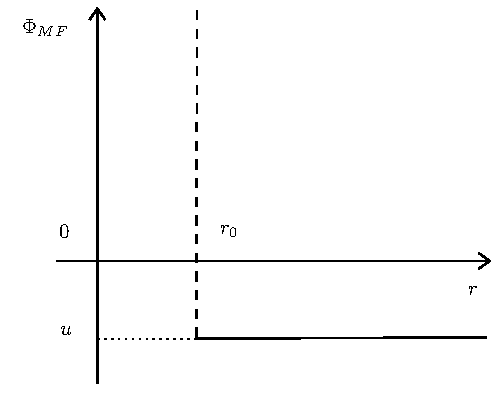
\includegraphics[width=0.6\textwidth]{../lessons/14_image/1.pdf}
\caption{\label{fig:} Description.}
\end{figure}

 What could be more reasonable as a potential is the Lennard-Jones, but it is not it.
Instead, we have
\begin{equation}
\Phi _{MF} =
  \begin{cases}
   \infty & r < r_0\\
   u < 0 & r> r_0
  \end{cases}
\end{equation}
\begin{equation}
  Q_N (T) = \qty[ (V-V_{ex})e^{-\beta u} ]^N
\end{equation}
where \( V_{ex} \sim r_0^3 \), the volume not accessible by the particle. The free energy is
\begin{equation}
  F_N = - N k_B T \qty[ \ln{(V-V_{ex})} - \beta u ]
\end{equation}
\begin{equation}
  P_N^{MF} = - \eval{\pdv{F_N}{V} }_T = \frac{N k_B T}{V-V_{ex}} - N \qty(\pdv{u}{V} )_T
  \label{eq:1}
\end{equation}
In general, the deep \( u \)  can go up and down depending on the \emph{V}: \( u = u (V) \). In principle, \( u \sim -N/V \). Where the density is very high you have more attraction.
It is expected that the volume not accessible \( V_{ex} = b N \), so \( u = - a N / V \). Inserting that term in \eqref{eq:1}, we obtain the Van der Walls:
\begin{equation}
  P_N (V,T) = \frac{N k_B T}{V-bN} - a \qty(\frac{N}{V})^2
  \label{eq:2}
\end{equation}
this is the Van der Walls. We have this effect because it is a mean field, so the curve in Figure 2 it is replaced by the curve in Figure 3.


\begin{figure}[h!]
\begin{minipage}[c]{0.5\linewidth}
\subfloat[][Description]{ 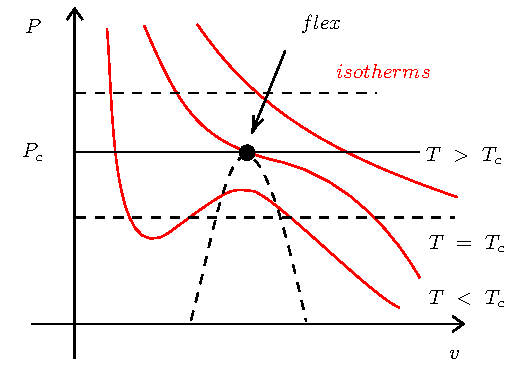
\includegraphics[width=0.8\textwidth]{../lessons/14_image/2.pdf}  \label{fig:} }
\end{minipage}
\begin{minipage}[]{0.5\linewidth}
\centering
\subfloat[][Description]{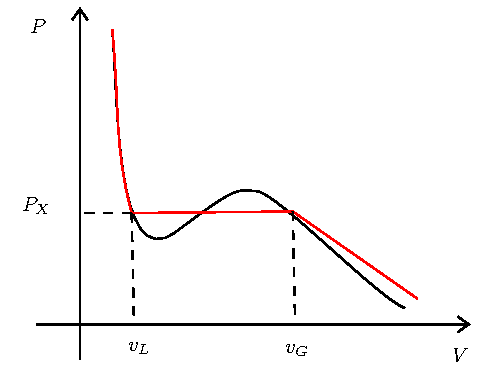
\includegraphics[width=0.8\textwidth]{../lessons/14_image/3.pdf}  \label{fig:} }
\end{minipage}
\caption{\label{fig:} Description}
\end{figure}




This two condition
\begin{equation}
  \pdv{P}{v} = 0 \qquad \pdv[2]{P}{v} = 0
\end{equation}
are the equation for finding the critical points. The second in particular means that there is a flex point. Pay attention to it, it is a standard way. The way used in the notes is slightly different.

We have  \( v_c = 3 b \):
\begin{equation}
  p_c = \frac{a}{27 b^2} \qquad k_B T_c = \frac{8a}{27b}
\end{equation}
so
\begin{equation}
  \frac{p_c v_c}{k_B T_C} \approx 0.375
\end{equation}
Nevetherless, if you compute the critical point and you compute this ratio you will obtain the same value.

Another way to rewrite \eqref{eq:2} is choosing
\begin{equation}
  \pi \equiv \frac{p}{p_c}, \quad \nu  \equiv \frac{v}{v_c}, \quad \tau \equiv \frac{T}{T_c}
\end{equation}
so
\begin{equation}
  \qty(\pi + \frac{3}{\nu ^2}) \qty(3 \nu -1) = 8 \tau
\end{equation}
Try to do the expansion around the critical point, \( t = \tau -1 = \frac{T-T_c}{T_c}\) and \( \Phi = \nu -1 = \frac{v-v_c}{v_c} \). You want the deviation from the critical point.


\begin{equation}
  Q_N (T) = \int_{V}^{} \prod_{i=1}^{N}  \dd[]{\va{r}}  \exp [-\beta \sum_{i,j > i }^{}  U_2 ( \abs{\va{r}_i - \va{r}_j} ) ]
\end{equation}

\begin{equation}
  Z_N = \frac{1}{N! \Lambda ^{3N} } Q_N
\end{equation}
For an ideal gas we have: \( Q_N = V^N \)
\begin{equation}
  \rightarrow Z_N^{ideal} = \frac{V^N}{N! \Lambda ^{3N}}
\end{equation}
Now, suppose that \( U_2 \neq 0  \) but small! We can say that we can assume that our \( Q_N (V,T) \) it would be the ideal version times a new function
\begin{equation}
  Q_N (V,T)=V^N \chi _N (V,T)
\end{equation}
so
\begin{equation}
  F_N = F_N^{ideal} - k_B T \ln{\chi _N}
\end{equation}
This also suggest, that you can formally expand the equation of state as a function of the density
\begin{equation}
  \frac{P}{k_B T} = \rho
\end{equation}
this is the ideal gas, now start to add the other terms of the expansion
\begin{equation}
  \rightarrow \frac{P}{k_B T} = \rho + B_2 (T) \rho ^2 + B_3 (T)\rho ^3+ \dots + O(\rho ^n)
\end{equation}
this is a \emph{virial expansion}, it is one of the most used. The coefficient \( B \) are called the \emph{virial coefficients}.  Making a fit, you will obtain the virial coefficients. This is what physicist have done for years. Mapping the coefficient with the real world experiments, you can find some macroscopical parameters.

\begin{equation}
  \frac{P}{k_B T} = \frac{N}{V-bN} - \frac{a N^2}{k_B T V^2}
\end{equation}
do an expansion, you will get the same structure of the virial expansion, finding the virial coefficient of the Van der Walls. Therefore,
\begin{equation}
  B_2 (T)^{VdW} = b - \frac{a}{k_B T} \qquad B_3^{VdW} = b^2
\end{equation}
The \emph{Boyle's temperature} is when the second coefficient is zero:
\begin{equation}
  B_2^{VdW} (T_B) = 0
\end{equation}
so you remove the most important coefficient.
We have \( T_B \) versus \( T_c \). It is clear that the Boyle's temperature must be much greater than the critical one. Consider a polymer, the transition point called the \( \theta  \) point is when the second coefficient is zero, as the case described above, but it is interesting in polymer kind of system.

Let us try to do some calculation of this virial coefficients, starting from the model microscopical
\begin{equation}
  Q_N = \int_{V}^{} \dd[]{\va{r}_1} \dots \int_{V}^{} \dd[]{\va{r}_N}  e^{-\beta \sum_{i,j > i}^{} \Phi _{ij} }
\end{equation}
with
\begin{equation}
  \Phi _{ij} = \Phi ( \abs{\va{r}_i - \va{r}_j} )
\end{equation}
The \emph{Mayer function}  is something that is smaller in that given point
\begin{equation}
  f (\abs{\va{r}} ) \equiv \exp [ - \beta \Phi ( \abs{\va{r}} )] -1
\end{equation}
If \( \beta \Phi \ll 1 \), we have \( f \ll 1 \). So
\begin{equation}
  \rightarrow  e^{-\beta \sum_{i,j > i}^{} \Phi _{ij} } = \prod_{i}^{} \qty(\prod_{j>i}^{} (1+ f_{ij})  )
\end{equation}
Expanding this object we obtain
\begin{equation}
  \rightarrow = \underbrace{(1+f_{12})(1+f_{13}) (1+ f_{14}) \dots ( 1 + f_{1N })}_{i=1}   \dots \underbrace{(1+f_{23}) (1+ f_{24}) \dots ( 1 + f_{2N })}_{i=2} \dots =
\end{equation}
\begin{equation}
  = 1 + \sum_{i}^{} \sum_{j>i}^{} f_{ij} + \cancel{\sum_{i}^{} \sum_{k \ge i}^{} \sum_{j > i}^{} \sum_{e \ge j}^{} f_{ik} f_{je}       }  
\end{equation}
The solution is given by considering only the linear term. This is the cluster expansion.



\end{document}
